\chapter{Metodologia}
\label{cap:03}

Para que seja possível cumprir os objetivos desse trabalho de conclusão de curso, no presente capítulo serão apresentados todos os passos a serem desenvolvidos. Todos os trechos de código utilizados nesta seção para comparação entre as linguagens \textit{Kotlin} e \textit{Java} apresentam-se disponíveis para visualização e consulta no sistema de gerenciamento e versionamento de projetos \textit{GitHub} no endereço \url{https://github.com/wendreof/tcc}.

Para a organização dos códigos utiliza-se as formatações, endentações e otimização de importações oferecidas pela própria \textit{IDE Android Studio} e para a estruturação dos projetos utiliza-se o padrão de desenvolvimento com nomenclatura de classes, variáveis, operações e relacionados somente na língua inglesa. Em cada um dos experimentos, explica-se de forma resumida o conteúdo de cada trecho de código, e as particularidades referentes, principalmente ao \textit{Kotlin}, pois o presente trabalho não tem por objetivo, se aprofundar em todos os conceitos relacionados às tecnologias aplicadas.

Todos os comentários utilizados nos trechos de códigos no decorrer do capítulo, apresentam-se sem seus devidos acentos e pontuações, devido a falta de compatibilidade com o Formato de Transformação Unicode 8-bit (\textit{Unicode Transformation Format – 8-bit - UTF-8}).

\section{Panorama Geral da Pesquisa}

O panorama geral desta pesquisa, conforme representado a seguir na Figura 9, propõe-se a esclarecer o motivo da escolha da apresentação de uma nova tecnologia para o desenvolvimento de \textit{software} voltado para os dispositivos móveis por meio de métricas para comparação entre duas linguagens de programação, sendo elas \textit{Java} e \textit{Kotlin}, que por sua vez fazem parte do ecossistema da plataforma móvel \textit{Android} e o desenvolvimento e análise de experimentos baseados em trechos de códigos que desempenham as mesmas funcionalidades.

\FloatBarrier
\begin{figure*}[!htbp]
	\centering
		\caption{Panorama Geral da Pesquisa}
	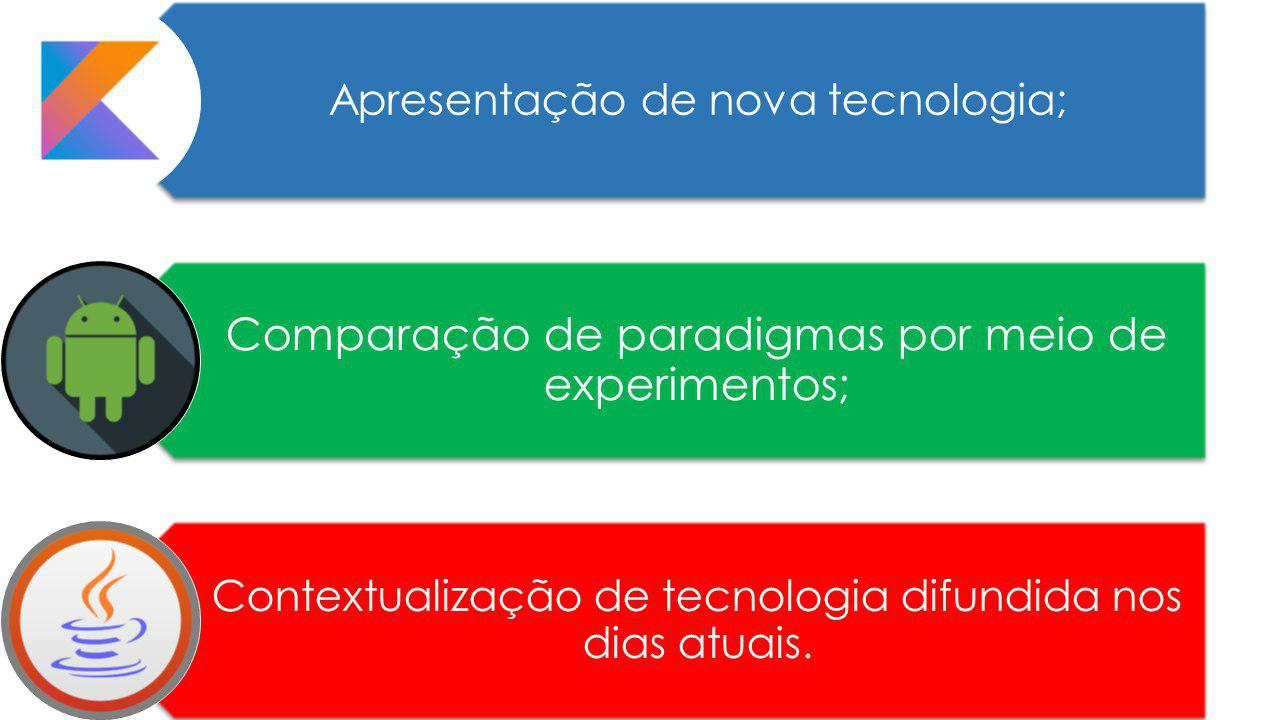
\includegraphics[scale=0.5]{imagens/metodologia1}
	\subcaption{\textbf{Fonte:} Elaborado pelo autor}
	\label{fig:figura3}
\end{figure*}
\FloatBarrier

De acordo com o panorama geral da pesquisa, apresentado na Figura 9 acima, a seguir listam-se todas as etapas a serem operacionalizadas, para cumprir-se os objetivos gerais e específicos deste trabalho de conclusão de curso.

\begin{itemize}
    \item \textbf{Etapa 01}: Justificativa para Adoção do \textit{Kotlin} com Destaque nos Aspectos de Usabilidade;
    
    \item \textbf{Etapa 02}: Métricas de Usabilidade para Comparação;
    
   \item \textbf{Etapa 03}: Definição de Experimentos para Comparação entre \textit{Kotlin} e \textit{Java};

   \item \textbf{Etapa 04}: Comparação entre as Linguagens Kotlin e Java para os Experimentos Definidos.
\end{itemize}

\section{Etapas para o Desenvolvimento da Pesquisa}

\subsection{Etapa 01: Justificativa para Adoção do \textit{Kotlin} com Destaque nos Aspectos de Usabilidade}

Como reforçado nos capítulos anteriores dessa pesquisa, mais especificamente no segundo capítulo, a linguagem de programação Java ainda é o principal e mais utilizada para desenvolvimento de aplicações móveis destinadas para os usuários do sistema operacional \textit{Android}. Desde seu anúncio oficial, o \textit{Kotlin} chegou para oferecer aos desenvolvedores mais uma opção no momento de escolha de tecnologias para elaboração de novos aplicativos assim como a manutenção de sistemas legados, ou seja, \textit{Kotlin} não vai e nem pretende substituir o \textit{Java}, mas sim \textbf{coexistir} de forma homogênea no ecossistema \textit{Android}. Munido de recursos mais modernos, inspirados em tecnologias reconhecidas no mercado de desenvolvimento de software, com \textit{Kotlin} torna-se possível escrever algoritmos compreendidos pela \textit{JVM}, de modo mais simples, facilitando todas as etapas que envolvem a programação e possibilitando o aproveitamento de tudo que já foi escrito em \textit{Java} como classes, projetos e bibliotecas.

Ao término da pesquisa, pretende-se evidenciar as vantagens da programação com foco em dispositivos móveis, utilizando como principal tecnologia, a linguagem de programação \textit{Kotlin}, apoiando-se em seus aspectos modernos e enxutos, resultando em uma menor quantidade de código clichê e desnecessário que em nada auxiliam a aplicação e acabam dificultando a manutenção.

\subsection{Etapa 02 - Métricas de Usabilidade para Comparação} 
Baseando-se em um dos conceitos descritos pelo escritor e engenheiro de \textit{software} americano Robert C. Martin, autor do renomado livro \textit{Clean Code: A Handbook of Agile Software Craftsmanship}, no qual se é descrito que na programação lê-se muito mais vezes do que se escreve um código propriamente dito, as etapas estabelecidas para equiparar \textit{Kotlin} e \textit{Java} são apresentadas na Tabela 2:

\FloatBarrier
\begin{table}[!htbp]
\centering
\caption{Métricas de comparação}
	\begin{tabular}{ c | c }
		\hline
		\textbf{Métrica} & \textbf{Definição}                  \\ \hline
		
		             1 	 & Quantidade de caracteres utilizados	\\ \hline
		             
		             2   & Quantidade de linhas de código        \\ \hline
		             
		         	 3   & Tamanho do arquivo em quilobytes (Kb) \\ \hline
	\end{tabular}
	\\ \vspace{0.2cm}
	\textbf{Fonte:} Elaborada pelo autor
	\label{tab:exemplo}
\end{table}
\FloatBarrier

%\begin{itemize}
%\    \item \textbf{Quantidade de caracteres}: Em uma linguagem de programação mais verbosa utiliza-se uma quantidade relativamente maior de caracteres e símbolos
    
%\     \item \textbf{Quantidade de linhas de código}: Em um código considerado verboso, encontra-se uma quantidade maior de palavras e/ou palavras mais longas para se expressar a intenção do algoritmo (consequentemente mais linhas)

%\     \item \textbf{Tamanho do arquivo em Quilobytes (Kb)}: Quanto maior o tamanho do arquivo (.java/.kt), maior será o tempo utilizado para ser efetuada a compilação pela \textit{JVM} %\\end{itemize}  

Em linguagens de programação mais verbosas, faz-se necessária a utilização de uma maior quantidade de caracteres e símbolos, da mesma forma podem-se aumentar a quantidade de palavras chaves e palavras mais longas que o normal para que se torne possível se expressar a real intenção de um algoritmo, o que gera a inclusão de mais linhas no projeto, e consequentemente aumenta o tamanho final do arquivo utilizado em caso de linguagens compiladas como o \textit{Java} e sua \textit{JVM}. Entende-se que uma determinada linguagem que necessita de menos de caracteres, expressões e linhas de código é menos verbosa, mais expressiva e de maior facilidade referente a sua manutenção.

Assim, para os experimentos desta pesquisa, ao comparar as linguagens \textit{Kotlin} e \textit{Java}, serão analisadas as métricas apresentadas na Tabela 2.

\subsection{Etapa 03 - Definição de Experimentos para Comparação entre \textit{Java} e \textit{Kotlin}}

Abaixo os experimentos a serem desenvolvidos no decorrer do capítulo para que seja possível atingir o objetivo de comparação:

\textbf{Experimento I} - \textit{Hello World}!: Apresentação de um pequeno trecho de código que ao ser executado, apresenta uma saída para o usuário;

\textbf{Experimento II} - Operação Aritmética Básica: Elaboração de uma função que tem por intuito realizar a somar de dois números inteiros e interpolar o resultado com um texto;

\textbf{Experimento III} - Classe \textit{Student}: Implementação de uma classe modelo que abstrai algumas das características presentes em um estudante;

\textbf{Experimento IV} - Classe \textit{ThermometricScale}: Apresentação da classe base para o desenvolvimento da aplicação de medidas termométricas e declaração de suas três funções;

\textbf{Experimento V} - Interface \textit{Temperature}: Implementação de uma interface e um método que recebe dois valores por parâmetros e retorna um único valor;

\textbf{Experimento VI} - Classe \textit{Adapter}:
Utilização das técnicas de se extender e implementar uma classe e uma interface;

\textbf{Experimento VII} - \textit{Activity Main}: Criação da principal classe da aplicação de conversão e implementação de todos os eventos de clique e substituição dos textos apresentados na interface.

Nos experimentos I, II, II trabalham-se trechos desconexos de códigos de caráter mais introdutórios das duas linguagens, entretanto, nos experimentos IV, V, VI e VII com o intuito de aprofundar-se mais especificamente na plataforma \textit{Android} e no seu ecossistema, apresentam-se duas classes, uma interface e uma terceira classe do tipo \textit{activity}, ambas referentes a uma aplicação que realiza a conversão de valores termométricos de acordo com o diagrama em Linguagem de Modelagem Unificada (\textit{Unified Modeling Language} - \textit{UML}) apresentado na Figura 10:

\FloatBarrier
\begin{figure*}[!htbp]
	\centering
		\caption{Diagrama \textit{UML} de Aplicação de Conversão de Medidas Termométricas}
	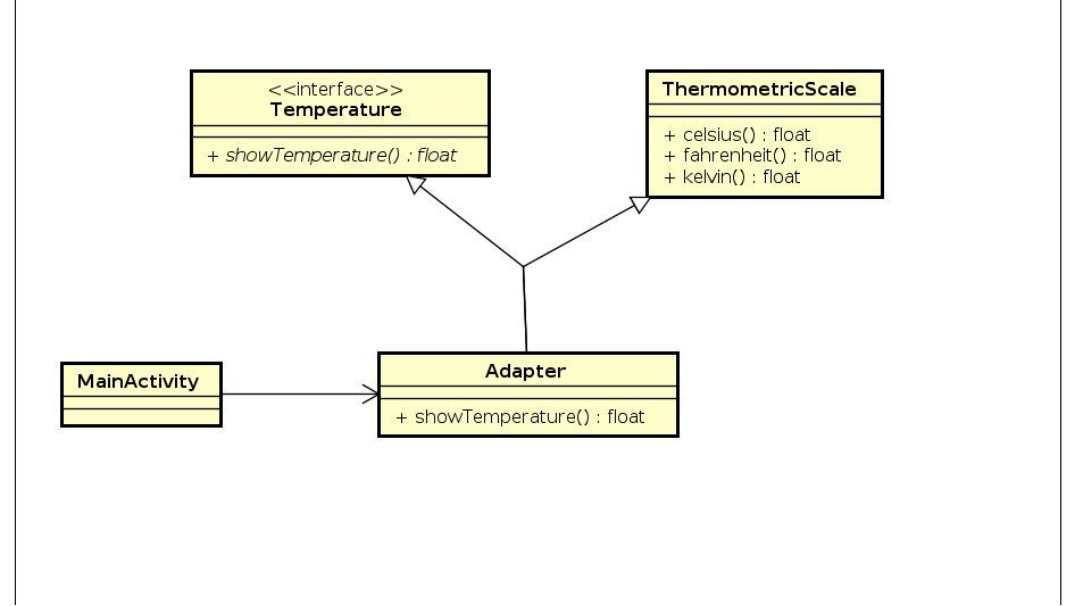
\includegraphics[scale=1]{imagens/umlTCC}
	\subcaption{\textbf{Fonte:} Elaborado pelo autor}
	\label{fig:figura3}
\end{figure*}
\FloatBarrier

No diagrama \textit{UML} disponibilizado na Figura 10 acima, apresenta-se um exemplo de implementação do padrão de projeto \textit{Adapter} em uma aplicação móvel, na Tabela 3 detalha-se cada uma das classes e suas respectivas funções:

\FloatBarrier
\begin{table}[!htbp]
\centering
\caption{Classes e Definições do diagrama UML - Figura 10}
	\begin{tabular}{ c | c }
		\hline
		\textbf{Classe} & \textbf{Definição}\\ \hline
		
         \textit{Adapter} & Adaptar a interface \textit{Temperature} e a classe \textit{ThermometricScale}
         \\ \hline
         
          \textit{Temperature}   & Definir a interface de domínio específica a ser adaptada
          \\ \hline
         
     	 \textit{MainActivity}  & Colaborar com objetos da a interface \textit{Temperature}
     	 \\ \hline
     	 
     	   \textit{ThermometricScale}  & Definir uma interface existente que necessita ser adaptada
     	   \\ \hline
	\end{tabular}
	\\ \vspace{0.2cm}
	\textbf{Fonte:} Elaborada pelo autor
	\label{tab:exemplo}
\end{table}
\FloatBarrier

\subsection{Etapa 04 - Comparação entre as Linguagens \textit{Kotlin} e \textit{Java} para os Experimentos Definidos}

\subsubsection{Experimento I - \textit{Hello World!}}

Como início da comparação, apresenta-se nessa subseção, duas versões de um \textit{Hello World}, que nada mais é, do que um trecho de código básico que normalmente é empregado de forma educacional para iniciantes para se exemplificar os princípios de uma determinada linguagem. A função de um \textit{Hello World} é exibir o texto \textit{Hello World!} (Olá Mundo!) de forma visual por meio de uma saída, seja ela \textit{IDE}, terminal ou tela.

Em versões anteriores do \textit{Kotlin}, fazia-se necessária a implementação de um parâmetro do tipo \textit{Array} de \textit{Strings} na função \textit{main} assim como faz-se necessário em \textit{Java}.


Exemplo de implementação de \textit{Hello World} em \textit{Kotlin}
\caption{Hello World em Kotlin}
\lstinputlisting[language=kotlin]{fontes/Main.kt} 

Exemplo de implementação de \textit{Hello World} em \textit{Java}
\caption{Hello World em Java}
\lstinputlisting[language=java]{fontes/Main.java} 


\subsubsection{Experimento II - Operação Aritmética Básica}

Nessa subseção, apresentam-se duas formas de se implementar a função aritmética de soma, declarando-se uma variável inteira que recebe a soma de dois valores inteiros, sendo eles os números 99 e 1 respectivamente, obtendo-se um total de 100. Os trechos de código após execução exibem um texto concatenando com a variável que recebeu o valor da soma.

Em Kotlin disponibilizam-se para utilização dois tipos de variáveis, sendo eles as variáveis mutáveis do tipo \textbf{\textit{var}} que podem ter seus valores alterados ao decorrer da execução do programa e as variáveis imutáveis do tipo \textbf{\textit{val}} que podem receber apenas uma atribuição de valor, sendo assim variáveis finais.

Exemplo de implementação de função aritmética de soma em \textit{Kotlin}
\caption{\textit{Hello World} em \textit{Kotlin}}
\lstinputlisting[language=Kotlin]{fontes/Operations.kt} 

Exemplo de implementação de função aritmética de soma em \textit{Java}
\caption{Hello World em Java}
\lstinputlisting[language=java]{fontes/Operations.java} 


\subsubsection{Experimento III - Classe \textit{Student}}

Nessa subseção foram implementam-se de formas diferentes uma mesma versão de uma classe \textit{Student} na qual implementam-se quatro atributos, sendo eles um atributo name do tipo \textit{string}, outro atributo denominado \textit{tccTitle} também do tipo \textit{string}, \textit{approved} do tipo \textit{boolean} e \textit{yearsOld} do tipo \textit{integer}, e as operações disponíveis são métodos acessores e de configuração \textit{getters} e \textit{setters}, \textit{toString}, \textit{equals} e \textit{hashCode}, todos eles comumente usados em classes do tipo \textit{Model} e na programação \textit{Java}.

Classes do tipo \textit{data class}  já possuem por padrão os métodos \textit{getter}, \textit{setter}, \textit{toString}, \textit{equals}, \textit{hashCode} e \textit{copy} implícitos, tornado desnecessária em \textit{Kotlin} a re-implementação das funções. Para obter-se um resultado parecido em \textit{Java} seria necessário configurar o \textit{Project Lombok} e utilizar as anotações \textit{@Getter}, \textit{@Setter}, \textit{@ToString} e \textit{@EqualsAndHashCode} ou a anotação \textit{@Data} no início da implementação da classe ou alguma outra ferramenta com o mesmo propósito.

Exemplo de implementação de uma classe \textit{Student} em \textit{Kotlin}
\caption{Exemplo de implementação de uma classe \textit{Student} em \textit{Kotlin}}
\lstinputlisting[language=kotlin]{fontes/Student.kt} 

Exemplo de implementação de uma classe \textit{Student} em \textit{Java}
\caption{Exemplo de implementação de uma classe \textit{Student} em \textit{Java}}
\lstinputlisting[language=java]{fontes/Student.java} 

\subsubsection{Experimento IV - Classe \textit{ThermometricScale}}

A classe \textit{ThermometricScale} não possui atributos, apenas três funções, sendo elas \textit{celsius}, \textit{fahrenheit} e \textit{kelvin}, cada uma das operações recebe e retorna um único valor do tipo \textit{float} que é utilizado na fórmula específica de cada uma das escalas termométricas implementadas.

Em \textit{Kotlin} é possível declarar uma função, seu tipo e respectivo retorno na mesma linha de forma mais simplificada e enxuta.

Classe \textit{ThermometricScale} em \textit{Kotlin}
\caption{\textit{ThermometricScale} em \textit{Kotlin}}
\lstinputlisting[language=kotlin]{fontes/ThermometricScaleKotlin.kt} 

Classe \textit{ThermometricScale} em \textit{Java}
\caption{\textit{ThermometricScale} em Java}
\lstinputlisting[language=java]{fontes/ThermometricScaleJava.java}

\subsubsection{Experimento V - Interface \textit{Temperature}}

A interface \textit{Temperature} possui apenas um único método denominado de \textit{viewTemperature}, que recebe por parâmetro um valor também do tipo \textit{float} e um único caractere.

Interface \textit{Temperature} em \textit{Kotlin}
\caption{Interface \textit{Temperature} em Kotlin}
\lstinputlisting[language=kotlin]{fontes/TemperatureKotlin.kt} 

Interface \textit{Temperature} em \textbf{\textit{Java}}
\caption{Interface \textit{Temperature} em \textit{Java}}
\lstinputlisting[language=java]{fontes/TemperatureJava.java} 


\subsubsection{Experimento VI - Classe \textit{Adapter}}

Na classe \textit{Adapter} implementada em \textit{Java}, torna-se necessária a criação da variável auxiliar r do tipo \textit{Float}, para que seja possível atribuir e retornar ao final da estrutura de decisão condicional \textit{Switch} o valor de forma correta. No entanto, na implementação em \textit{Kotlin}, a própria estrutura \textit{When} responsabiliza-se em retornar por padrão um valor, dispensando a criação de uma variável auxiliar.

A expressão \textit{when} está para a linguagem \textit{Kotlin} assim como \textit{If} e \textit{Switch} estão para o \textit{Java} e todas as demais linguagens derivadas da linguagem de programação \textit{C}.


\textit{Adapter} em \textit{Kotlin}
\caption{\textit{Adapter} em \textit{Kotlin}}
\lstinputlisting[language=kotlin]{fontes/AdapterKotlin.kt} 

\textit{Adapter} em \textit{Java}
\caption{\textit{Adapter} em \textit{Java}}
\lstinputlisting[language=java]{fontes/AdapterJava.java} 


\subsubsection{Experimento VII - \textit{Activity Main}} 

As duas versões de classe \textit{Activity Main} (classe principal) apresentadas a seguir, são de usabilidade simples e possuem como principal responsabilidade dentro do contexto da aplicação de conversão de medidas termométricas, capturar (vincular-se com) todos os \textit{widgets} (objetos/ferramentas) declarados no respectivo arquivo de Linguagem de Marcação Extensível (\textit{Extensible Markup Language - XML}) utilizado na interface, assim como todas as funções de clique em botões como o de limpar tela e converter a temperatura, \textit{Radio Buttons} para escolha de apenas uma única medida termométrica por vez seja ela \textit{Fahrenheit} ou \textit{Kelvin}, a apresentação/substituição de caixas de textos em campos do tipo \textit{EditText} e \textit{TextView}, exibição de mensagens para auxiliar o usuário na usabilidade da aplicação por meio de \textit{Snackbar} (caixas de textos temporárias na parte inferior do dispositvo) e por fim a validação (verificar se há um texto/valor presente) da caixa de texto do tipo \textit{EditText} na qual o usuário deve inserir um determinado valor em \textit{Celsius}.

Conforme apresentado na Tabela 3, a classe \textit{Activity Main} dada a estrutura do projeto, tem por obrigação colaborar em conformidade com todos todos os objetos da interface \textit{Temperature}.

\textit{Activity Main} em \textit{Kotlin}
\caption{Activity Main em Kotlin}
\lstinputlisting[language=kotlin]{fontes/MainActivityKotlin.kt} 

\textit{Activity Main} em \textit{Java}
\caption{Activity Main em Java}
\lstinputlisting[language=java]{fontes/MainActivityJava.java} 

\subsubsection{Aplicação de Conversão de Medidas Termométricas em \textit{Java} e \textit{Kotlin}}

Como resultado dos códigos desempenhados nesta seção, obtém-se as aplicações demonstradas na Figura 11 e Figura 12, referentes ao \textit{Java} e \textit{Kotlin}, respectivamente.
A aplicação de conversão de temperatura encontra-se disponível para \textit{download} na \textit{Play Store}, através do \textit{link} \url{https://bitlybr.com/qAwN7}

\FloatBarrier
\begin{figure*}[!htbp]
	\centering
		\caption{Aplicação de Conversão de Medidas Termométricas escrito em \textit{Java}}
	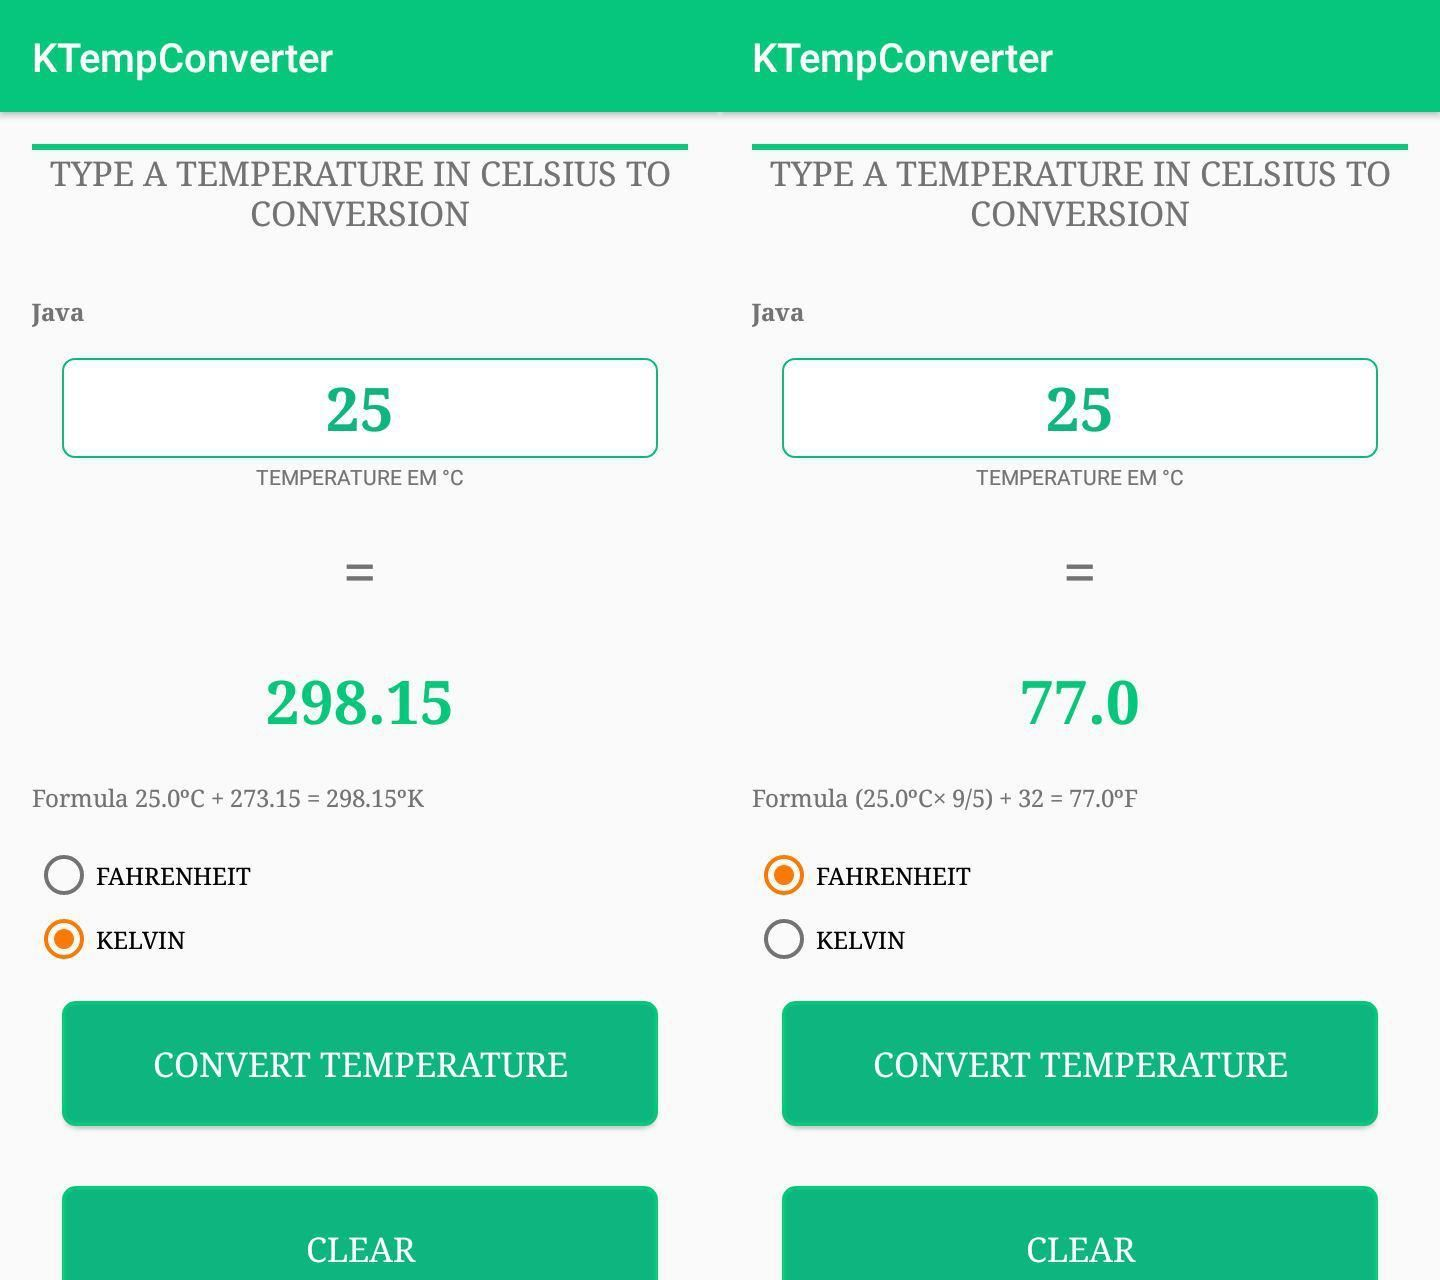
\includegraphics[scale=0.3]{imagens/java}
	\subcaption{\textbf{Fonte:} Elaborado pelo autor}
	\label{fig:figura3}
\end{figure*}
\FloatBarrier

As duas aplicações desempenham as mesmas funções e possuem os mesmos comportamentos, características e também o mesmo \textit{layout} (cores e disposição).  

\FloatBarrier
\begin{figure*}[!htbp]
	\centering
		\caption{Aplicação de Conversão de Medidas Termométricas escrito em \textit{Kotlin}}
	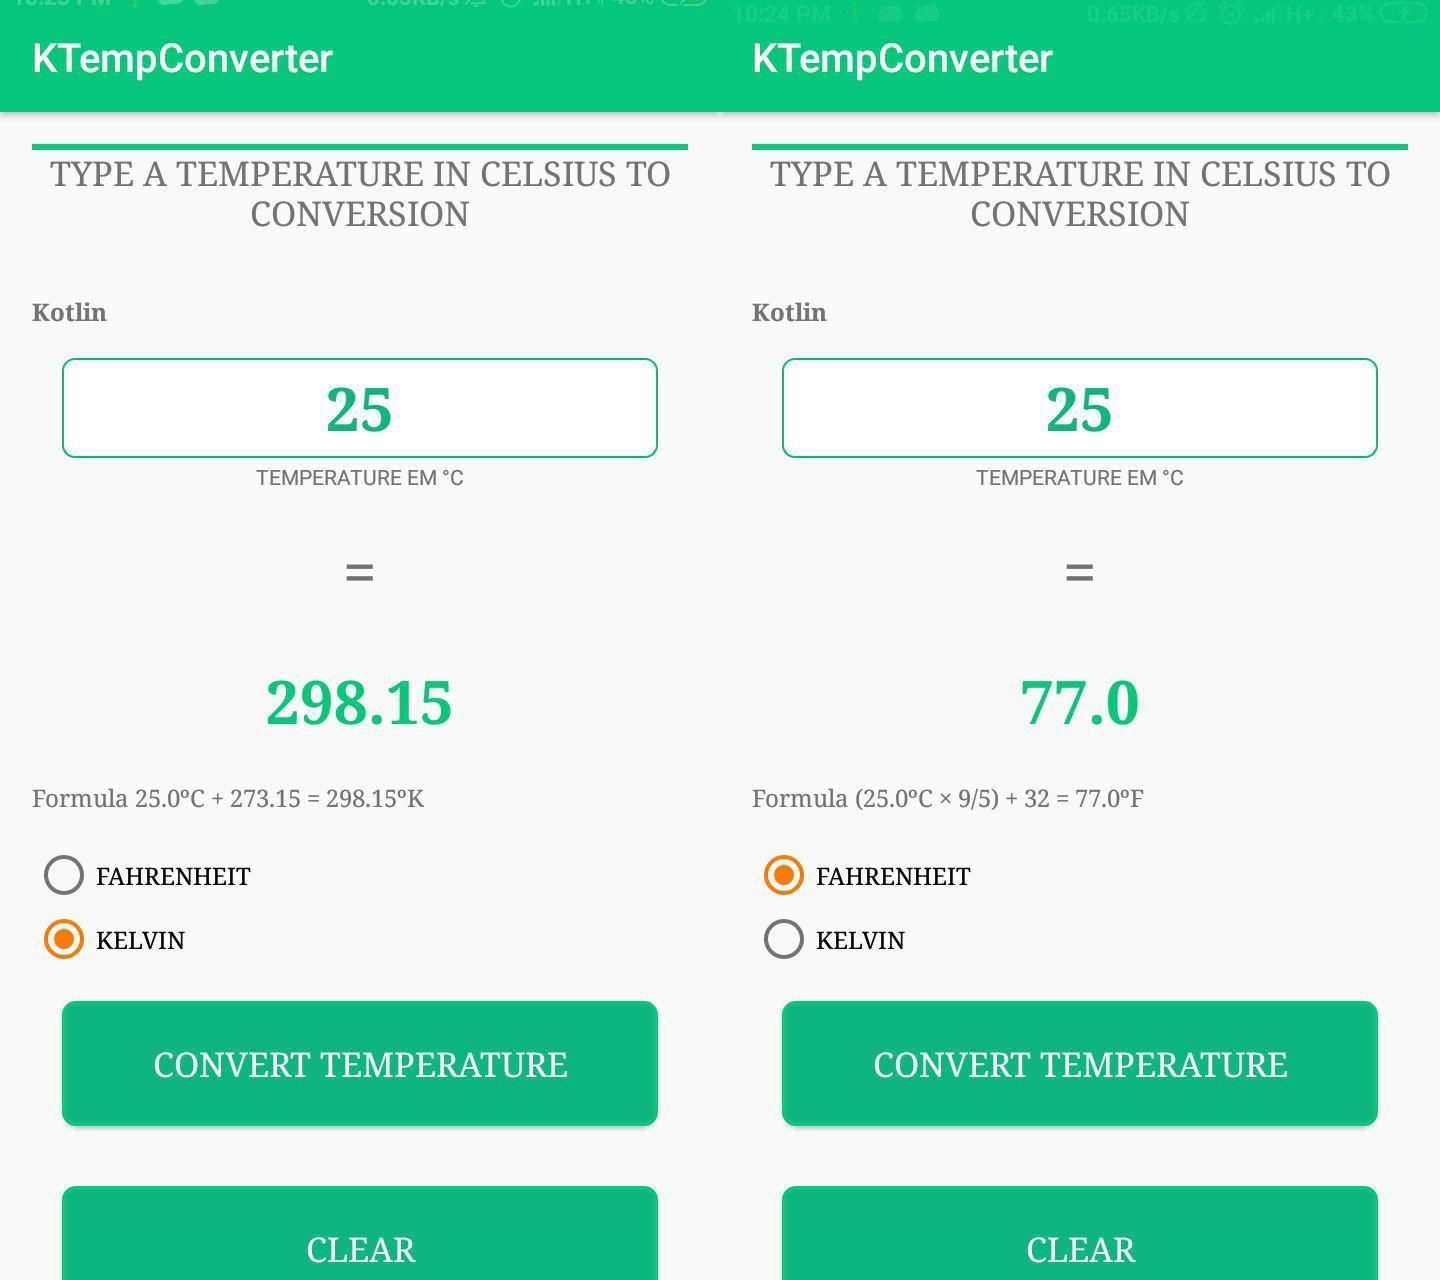
\includegraphics[scale=0.3]{imagens/kotlin}
	\subcaption{\textbf{Fonte:} Elaborado pelo autor}
	\label{fig:figura3}
\end{figure*}
\FloatBarrier

Tanto a aplicação \textit{Java} como a aplicação \textit{Kotlin} são capazes de realizar a conversão de uma medida em \textit{Celsius} inserida pelo usuário para \textit{Fahrenheit} ou \textit{Kelvin}.